\index{Wagner, Veit}
\subsubsection{Molecular and Nanoelectronics}

\paragraph{Research Team}
Veit Wagner (Professor),  Torsten Balster (Research Associate),
J\"{o}rg Seekamp (Research Associate), Arne Hoppe (PhD Student),
Benedikt Gburek (PhD Student), Sidhant Bom (Master Student) \ \ \\
\

%%% give a very short (150 words description of your research area)

Electronic devices based on semiconductors formed by organic molecules
are the focus of our research group. Transistors built from organic
materials allow extreme cheap production as well as new applications
like the use of bendable foils as transistor substrates. Furthermore,
shrinking of spatial dimensions to the length scale of individual
organic molecules (i.e. nanometer-scale) enables qualitatively new
device concepts, like the monolayer transistor or molecular
electronics devices. In the latter case individual molecules are used
as transistors or diodes. Goal of the research is the understanding of
the electronic transport mechanism in organic materials, at interfaces
involved and across molecular junctions. This includes testing of new
(molecular) device concepts and electronics at length scales below
those of state-of-the-art silicon electronics.

\paragraph{Highlights}

%%% give a short (500 words)description of the research highlights. 1 figure costs 100 words

Main advantages attributed to organic device concepts (organic
radio-frequency information tags (RFID), organic solar cells,
etc.) are the potentially very low productions costs, the low
processing temperatures and the option for wet-chemical
manufacturing. Due to the generally low carrier mobilities in
organic materials organic devices are restricted to low-frequency
applications so far. In 2006 in a systematic approach by shrinking
the channel lengths of {\it organic field-effect transistors
(OFET)} we were able to manufacture the {\it world-wide fastest
polymer transistor} reported so far~\cite{Wagner06-3,Wagner06-4}.
The device realized in bottom-contact configuration based on the
regio-regular polymer poly-hexylthiophene (P3HT, see
Fig.~\ref{fig:wagner1}) achieved a unity-gain bandwidth of 2~MHz
at a low driving voltage of 10~V and a channel length of 480~nm.
While these values wouldn't be a challenge for crystalline silicon
devices they are extremely high for wet-chemically processable
semiconductors. Furthermore, during this research work we could
identify contact resistance at the metal-organic interface as main
hindrance towards even higher frequencies predicted for lower
channel lengths, e.g. for a 120~nm device shown in
Fig.~\ref{fig:wagner1}. While contact properties require for
further optimization, MHz organic field-effect transistors will
open new areas of applications. Their large-scale production will
depend on upscaling of low-cost printing techniques, e.g.
micro-contact printing or nano-imprint lithography.

\begin{figure}[ht]
  \begin{center}
    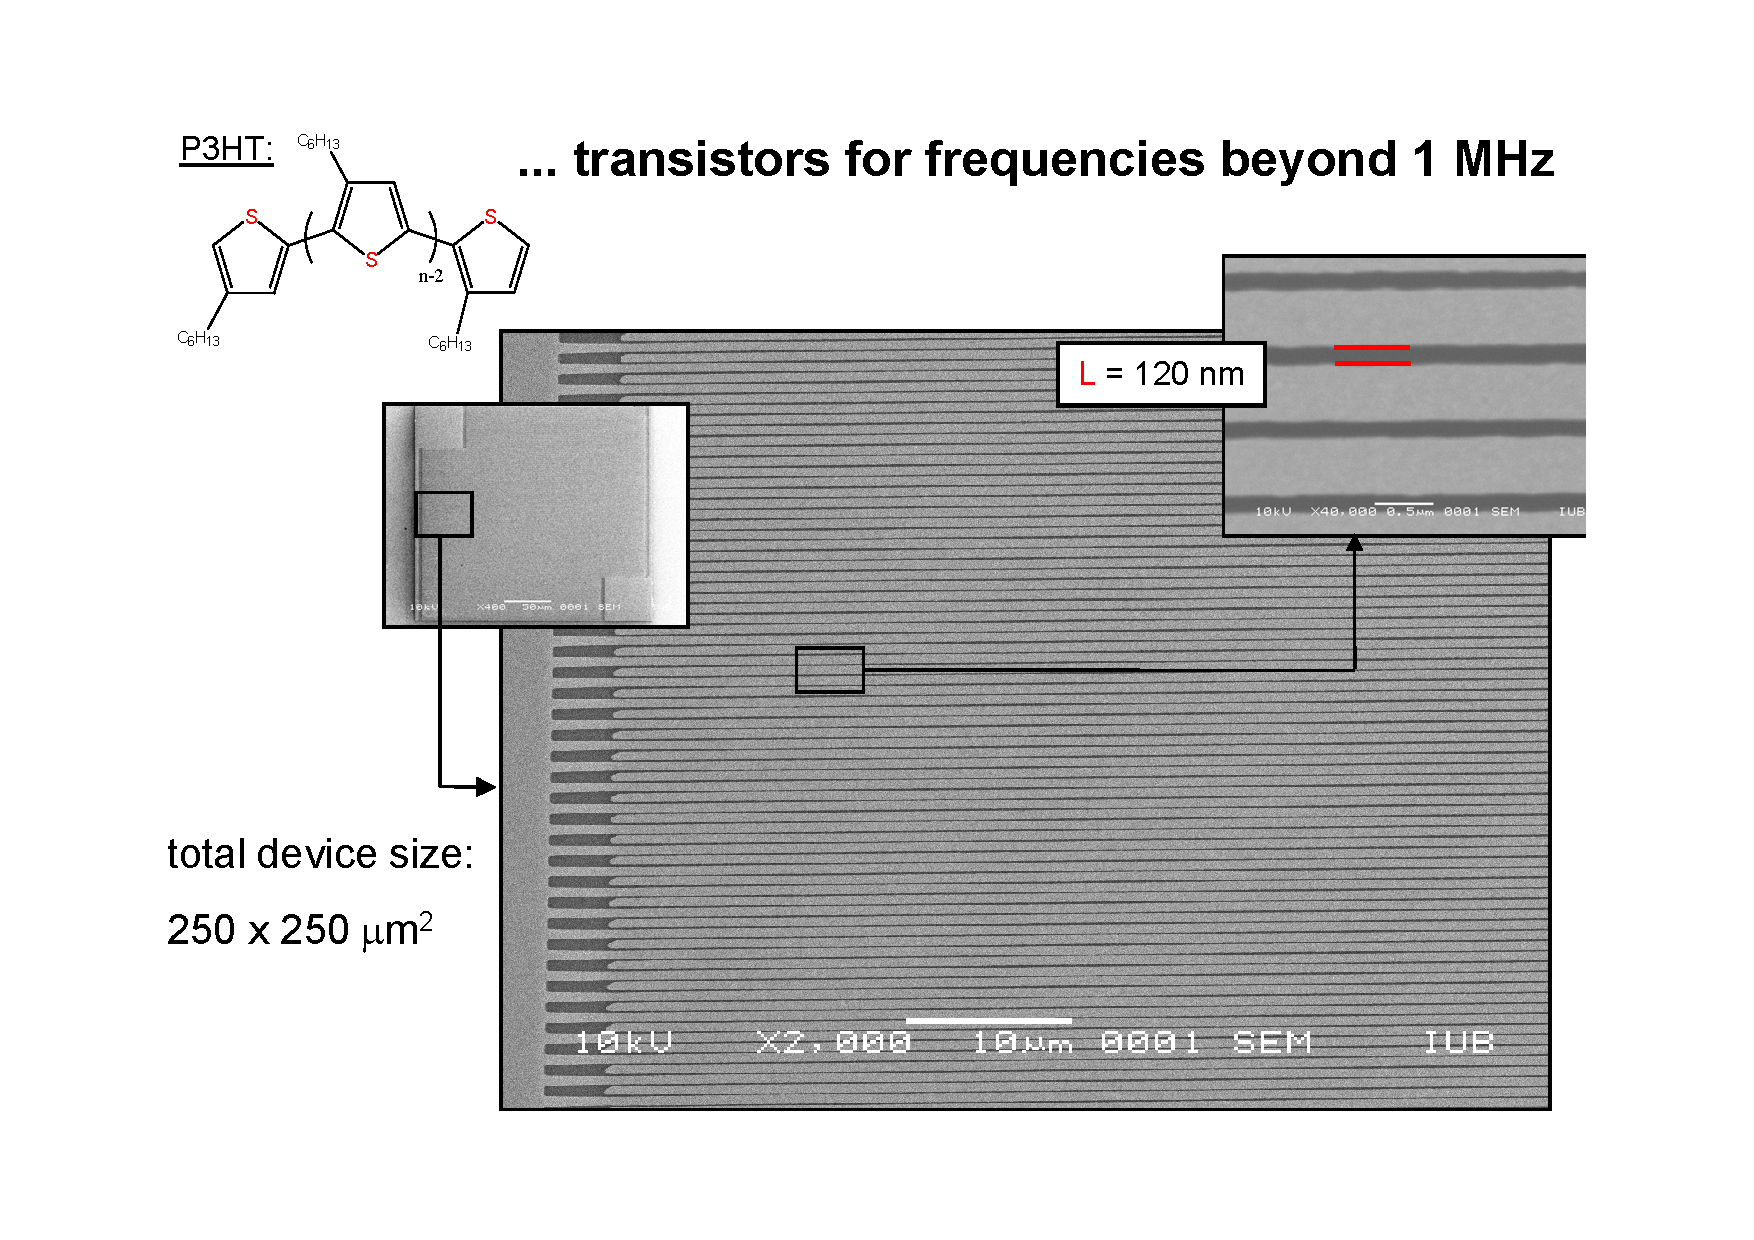
\includegraphics[width=6cm]{Wagner/Wagner_2006_Fig1.pdf}
    \caption{Polymer P3HT structure formula (upper left corner) and
     a top view of a L~=~120~nm transistor structure prepared by e-beam lithography on an oxidized
      silicon wafer (main part). Light grey areas show the interdigitated gold electrodes
       (source {\&} drain) and the dark areas are the SiO2 gate dielectric.
      The design allows for high current levels and small parasitic capacitances and
       is suitable to reach high frequencies.}
    \label{fig:wagner1}
  \end{center}
\end{figure}

Beside polymers also films consisting of small organic molecule
can be utilized as active semiconductor compound in devices, as
their are thiophenes or pentacene. Their crystalline ordering
results in better defined systems and higher carrier mobilities.
Main goal of the research is to understand and optimize contact
properties and aging behavior, e.g. {\it almost ideal contact
properties could be found for the system dihexyl-7-thiophene and
gold}. A very fruitful cooperation was established in this area
with the group of Prof. Knipp (IUB) for pentacene-based
devices~\cite{Wagner06-2}.

% to include a figure, generate a file xxx.pdf and integrate the following lines
% to reference it use ``Figure.~\ref{fig:xxx}''; the numbers will be computed automatically.
\begin{figure}[ht]
  \begin{center}
    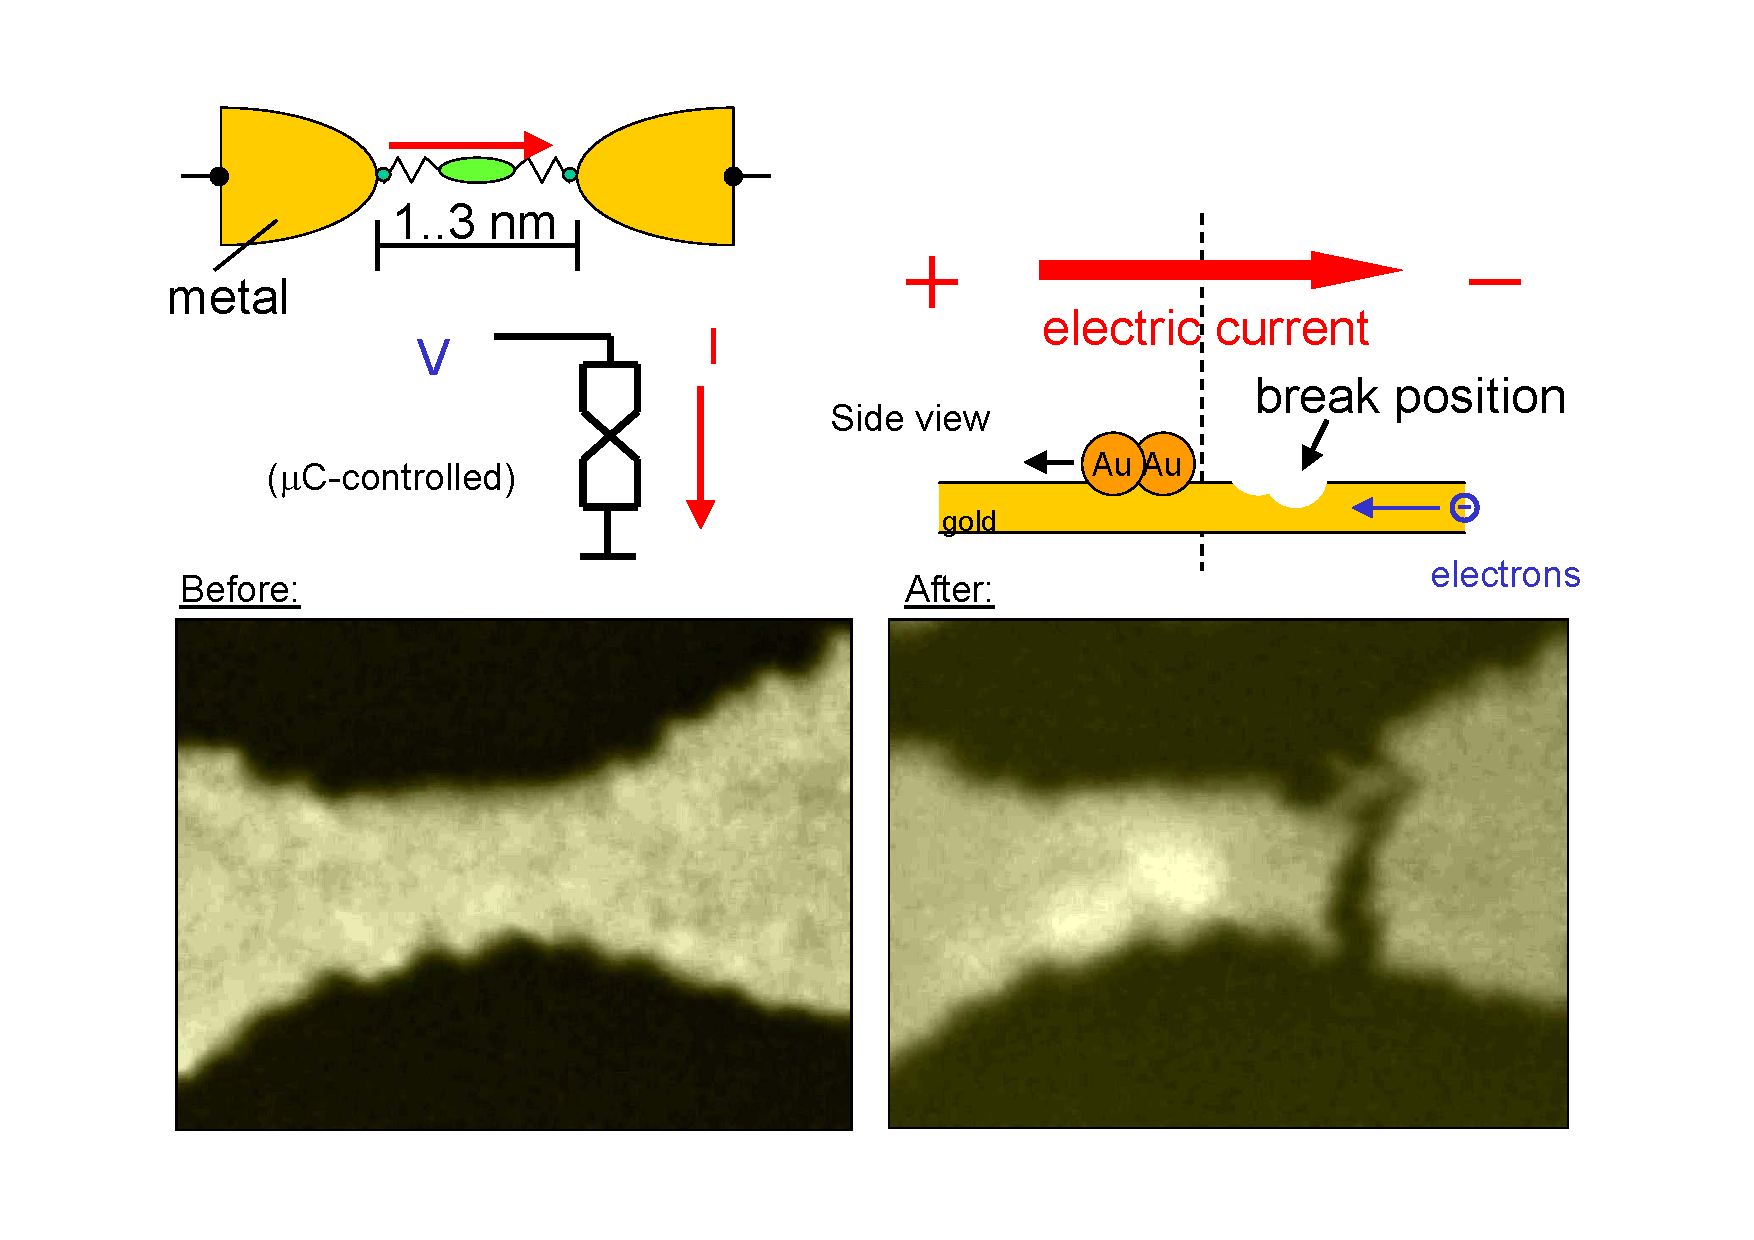
\includegraphics[width=\hsize]{Wagner/Wagner_2006_Fig2.pdf}
    \caption{Molecular electronics: a contacted single molecule (upper part). Below the
     electromigration set-up and the principle of operation (pushing the gold atoms by electrons).
     The lower part shows scanning electron micrsocope (SEM)
     images of a gold nano wire (width ca.~100~nm) before and
     after the elctromigration process.}
    \label{fig:wagner2}
  \end{center}
\end{figure}

A further research highlight is the successful preparation of
nano-sized electrodes (Fig.~\ref{fig:wagner2}) to contact
individual molecules utilizing an electromigration technique. In
this approach an increasing electric current level is imposed on a
lithographically defined gold nanowire until the wire breaks.
Small gaps comparable to the size of individual molecules, i.e.
1\dots 3 nm, can be realized via this technique. This approach was
enabled by the development of self-made electronics including a
fast microcontroller for realizing the feedback loop to control
the applied voltage, which allows to stop this process at any time
and gap size.


\paragraph{Organization}
% list the (research) events you have organized, if any,
\begin{enumerate}
\item Organization committee: European Summer School on Biosensing
  with channels: faster, smaller, smarter, 2006, IU-Bremen. %
\item Organization committee: Symposium Organic Thin Film
Electronics: From Molecular Contacts to Devices (SYOE), 2007, DPG annual meeting, Regensburg. %
\item Speaker of IUB graduate program Nanomolecular Science
\end{enumerate}

\paragraph{Collaborations}
\begin{enumerate}
\item {\sl International University Bremen}\\Prof. J{\"u}rgen
  Fritz\\AFM-Analysis, Bio-Molecules
\\Prof. Dietmar
  Knipp\\Micro-Contact Printing, Organic Transistors
\\Prof. Arnulf
  Materny\\Lithographically designed SERS-Substrates
\\Prof. Stefan
  Tautz\\Organic Molecules at Surfaces, Molecular Electronics
\item {\sl Universit{\"a}t Ulm}\\Prof. Peter B\"auerle\\Tailored
  Organic Molecules
\item {\sl ISAS-Berlin}\\Prof. Norbert Esser\\Surface Optics at
  Self-assembled Monolayers
\item {\sl Universit{\"a}t Bremen}\\Prof. Detlev Hommel\\Nano
  Lithography
\item {\sl Universit{\"a}t W{\"u}rzburg}\\Prof. Jean
  Geurts\\Characterization of Organic Transistors, Nano Lithography,
  Optical Analysis
\item {\sl ICMAB, Barcelona, Spain}\\Prof. David
  Amabilino\\Tetrathiafilvalenes (TTF) Molecules for Organic
  Electronics
\item {\sl Universidade do Algarve, Portugal}\\Prof. Henrique
  Gomes\\Electrical Analysis of Organic Transistors
\item {\sl Nova Gorica Polytechnic, Slovenia}\\Prof. Gvido
  Bratina\\Time-of-Flight Analysis and Theoretical Simulations of
  Organic Devices
\end{enumerate}

\paragraph{Grants}
% list the grants you have received in 2005, if none have been received, plese delete this
% subsection.
\begin{enumerate}
\item Funded by DFG, \emph{Organic field-effect transistors: scaling behavior
and
  interface properties} within Schwerpunktprogramm SPP 1121, Project WA 1039/2-1,2
  (January 2004 - December 2007)
\end{enumerate}

\paragraph{Other Support Grants}
% list the grants you have received in 2005, if none have been received, plese delete this
% subsection.
\begin{enumerate}
\item BMBF ''Embedded Microsystems Bremen (EMB)''
\end{enumerate}

%\paragraph{Awards, Prizes}
% list the grants you have received in 2005, if none have been received, please delete this
% subsection.
%\begin{enumerate}
%\item Selected as reviewer for the European Young Investigator
%Award
%  (EURYI)
%\end{enumerate}

%\paragraph{Publications}
% list the publications of 2005 (also accepted and in press), if none have been received, plese delete this
% subsection. Enter the publications into the SES publications database at
% http://kwarc.eecs.iu-bremen.de/ses-pubs/index.php and only reference them here.
%\begin{description}
%  \item[Journals]
\nocite{Wagner06-1} \nocite{Wagner06-2} \nocite{Wagner06-3}
\nocite{Wagner06-4} \nocite{Wagner06-5} \nocite{Wagner06-6}
%\end{description}
